% Created 2022-12-12 Mon 23:04
% Intended LaTeX compiler: pdflatex
\documentclass[a4paper,11pt]{article}
\usepackage[utf8]{inputenc}
\usepackage[T1]{fontenc}
\usepackage{graphicx}
\usepackage{longtable}
\usepackage{wrapfig}
\usepackage{rotating}
\usepackage[normalem]{ulem}
\usepackage{amsmath}
\usepackage{amssymb}
\usepackage{capt-of}
\usepackage{hyperref}
\usepackage[margin=1in]{geometry}
\usepackage{titlesec}
\usepackage{caption}
\usepackage{subcaption}
\usepackage{lipsum}
\author{Varghese Reji}
\date{}
\title{Classical and Quantum Optics\\\medskip
\large Assignment-2 Answers}
\hypersetup{
 pdfauthor={Varghese Reji},
 pdftitle={Classical and Quantum Optics},
 pdfkeywords={},
 pdfsubject={},
 pdfcreator={Emacs 28.2 (Org mode 9.5.5)}, 
 pdflang={English}}
\begin{document}

\maketitle

\section*{Problem 1}
\label{sec:org649bc04}

The python code to solve this question is given \href{https://github.com/varghesereji/Coursework\_assignments/blob/main/APP/Ass2/Problem\_1.py}{here}.


To create the upper confidence limit, we use the formula,

\begin{equation}
\label{eq:org1d2c5ae}
P(x<x_1|\mu)=1-\alpha
\end{equation}

and for central interval, we use

\begin{equation}
\label{eq:orgc53b20f}
P(x<x_1|mu)=P(x>x_2)=\frac{(1-\alpha)}{2}
\end{equation}

We will take the central interval 68\% and upper limit 90\%.

\begin{description}
\item[{(a)}] Poisson Discrete random variable.
\end{description}
\begin{equation}
\label{eq:orga8de30f}
P(x|\mu) = \frac{\mu^x}{x!}e^{-\mu}
\end{equation}

The plots are shown below.

\begin{center}
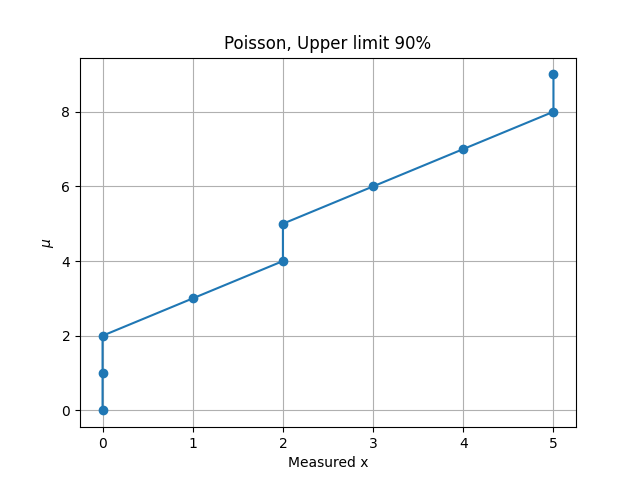
\includegraphics[width=.9\linewidth]{poisson_upper.png}
\end{center}

\begin{center}
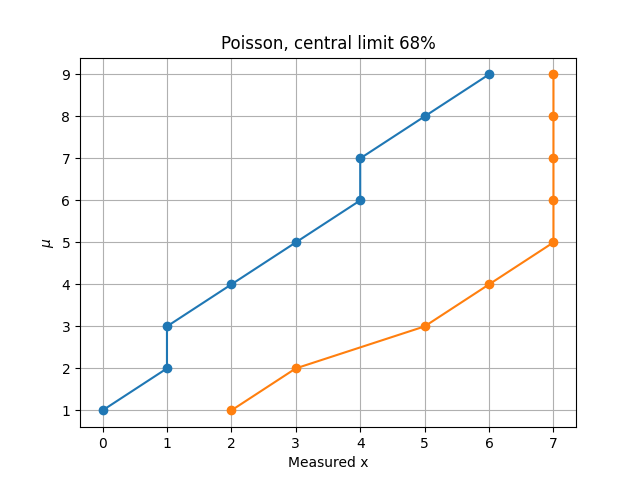
\includegraphics[width=.9\linewidth]{poisson_central.png}
\end{center}

\begin{description}
\item[{(b)}] Uniform distribution. Here, \(k=2\mu\).

Here, I took \(k=100\). Plots are shown here.
\begin{center}
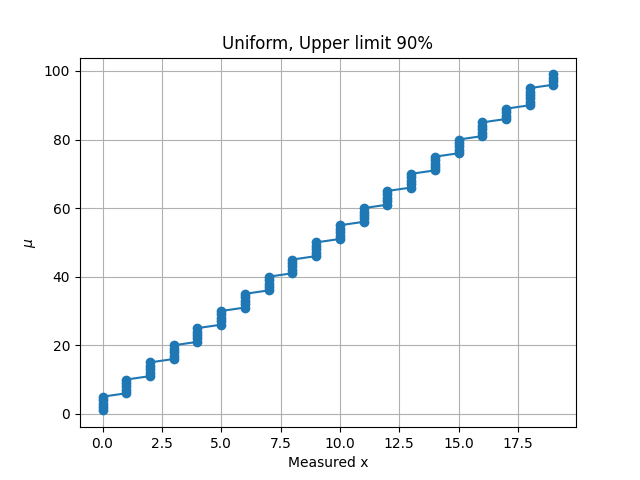
\includegraphics[width=.9\linewidth]{uniform_upper.png}
\end{center}

\begin{center}
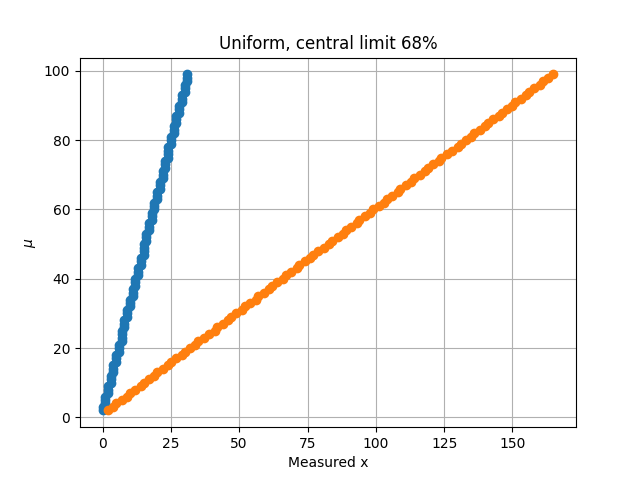
\includegraphics[width=.9\linewidth]{uniform_central.png}
\end{center}

\item[{(c)}] Gaussian function with \(\sigma=1\).
\end{description}


\begin{equation}
\label{eq:org0cbf9b2}
P(x|\mu) = \frac{1}{\sqrt{2\pi}} \exp\left(\frac{(x-\mu)^2}{2}\right)
  \end{equation}


\begin{center}
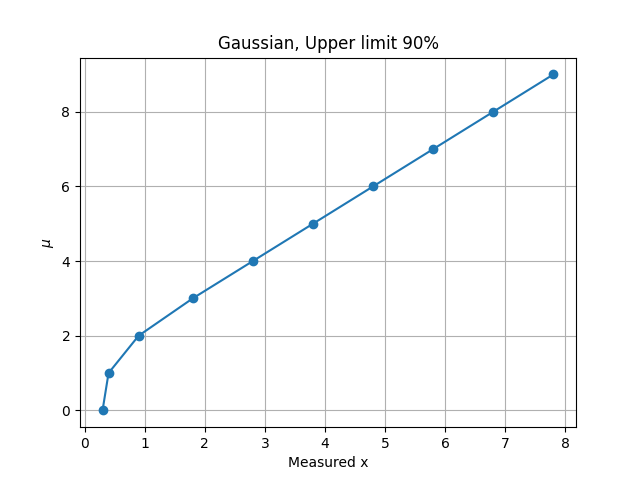
\includegraphics[width=.9\linewidth]{gaussian_upper.png}
\end{center}

\begin{center}
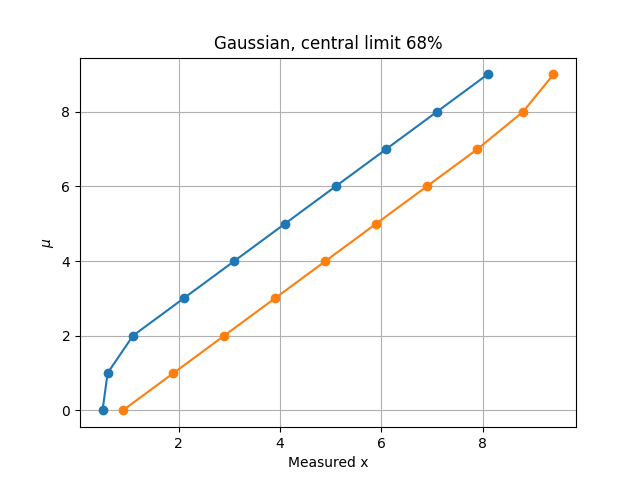
\includegraphics[width=.9\linewidth]{gaussian_central.png}
\end{center}

\section*{Problem 2}
\label{sec:org6c25263}

Let us consier an experiment done by Physicist X. He makes the following statements.
\begin{description}
\item[{(1)}] If the result \(x\) is less than 3\(\sigma\) , I will state an upper limit from the standard tables. If the result is less than 3\(\sigma\), I will state a central confidence interval from the standard tables.
\item[{(2)}] If my measured value of a physically positive quantity is negative, I will pretend that I measured zero when quoting a confidence interval.\cite{1998}
\end{description}

The first one is called 'flip-flopping'. Second one will introduce some conservatism. Using these statements, we can make the plot shown in fig \ref{fig:orgee24ce3}. For each value of the measured x, we can extimate the segment [\(\mu\)\textsubscript{1}, \(\mu\)\textsubscript{2}] by drawing a vertical line. Then we can examing the collection of vertical confidence intervals to see what horizontal acceptance intervals it implits. But in some cases, it does not satisfy the equation

\begin{equation}
\label{eq:orgbd0f265}
P(x\in[x_1, x_2]|\mu)=\alpha
\end{equation}

Suppose \$\(\mu\)=2.0, the accaptance interval has x\textsubscript{1}=2-1.28 and x\textsubscript{2}=2+1.64. But this interval only contains 85\% of the probability. That means, \ref{eq:orgbd0f265} is not satisfied. The interval is undercover for a significant range of \(\mu\): they are not confidence intervals or conservative confidence intervals.

But without flip-flopping, using the second statement only, the result will be unsatisfying when we get x as negative values. In that case, when we draw a vertical line as directed and finds that the confidence interval in empty set. So these are the issues we are facing at the moment, and these can be solved by using ordering principle. That's why ordering principle is relevant.
\begin{figure}[htbp]
\centering
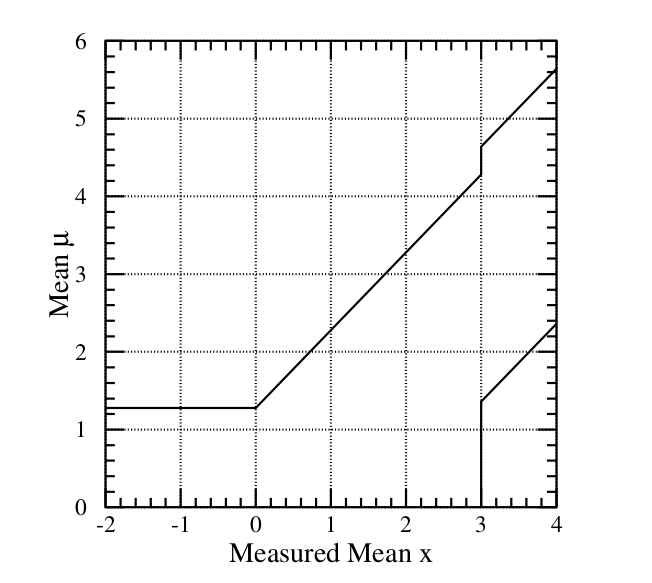
\includegraphics[width=.9\linewidth]{fig_4.png}
\caption{\label{fig:orgee24ce3}Plot of confidenc belts made based on statements. \cite{1998}}
\end{figure}


\section*{Problem 3}
\label{sec:org311d280}
Here, we use a backgroung b=3.0. ( It is mentioned in the paper). Values of \(\mu\) is from 0 to 50 with an interval 0.5.

The plots are shown below.

\begin{center}
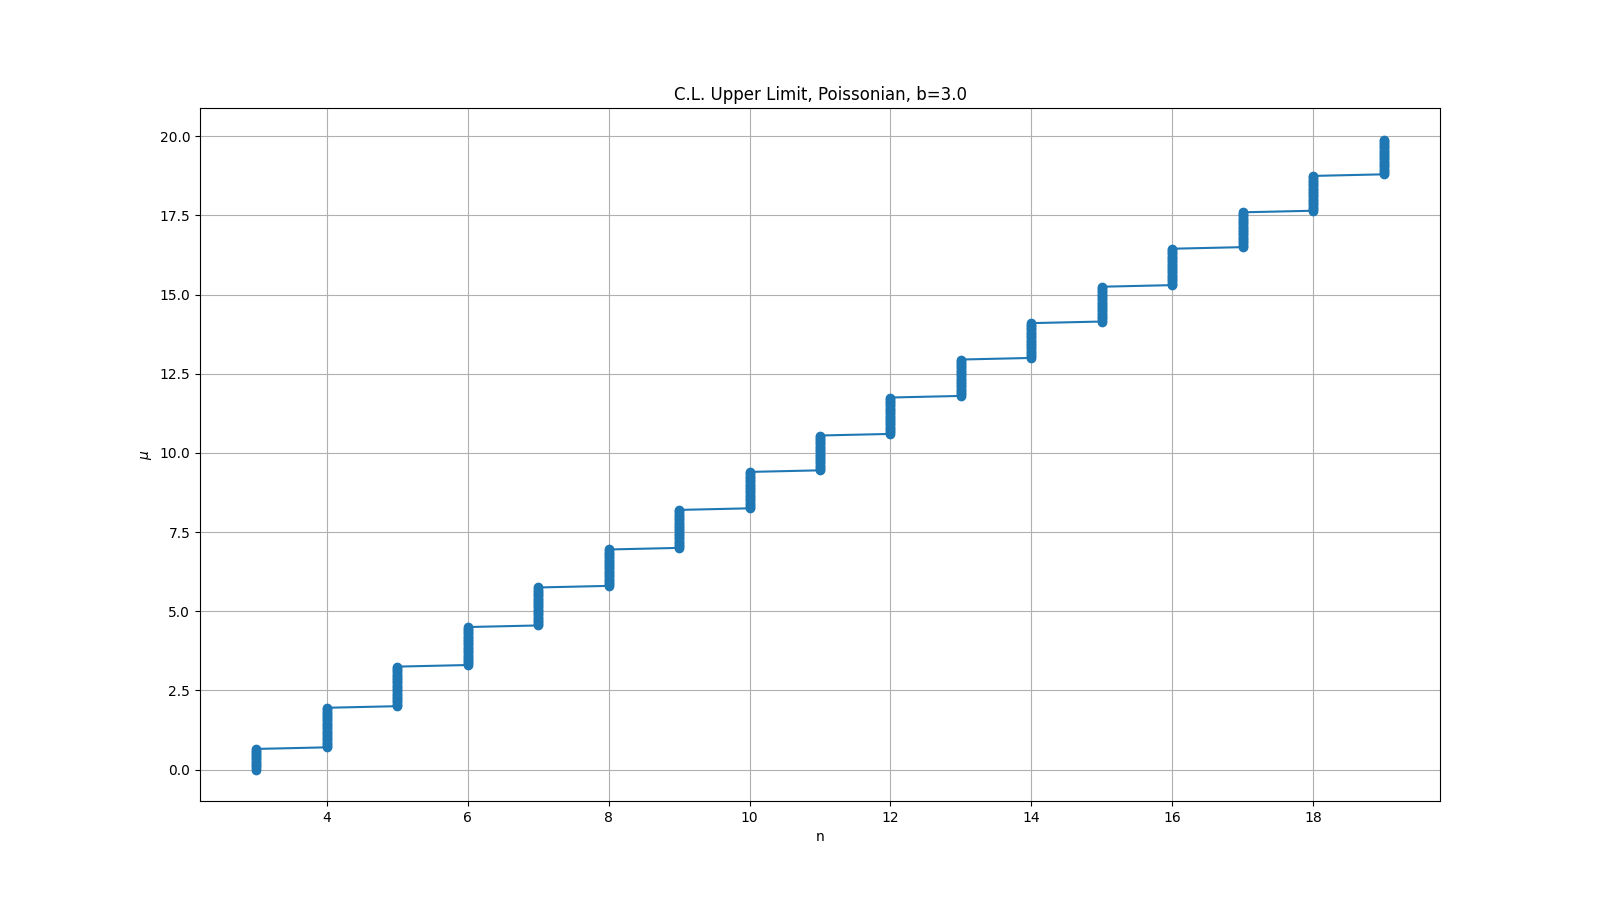
\includegraphics[width=.9\linewidth]{pr3_ul.png}
\end{center}

\begin{center}
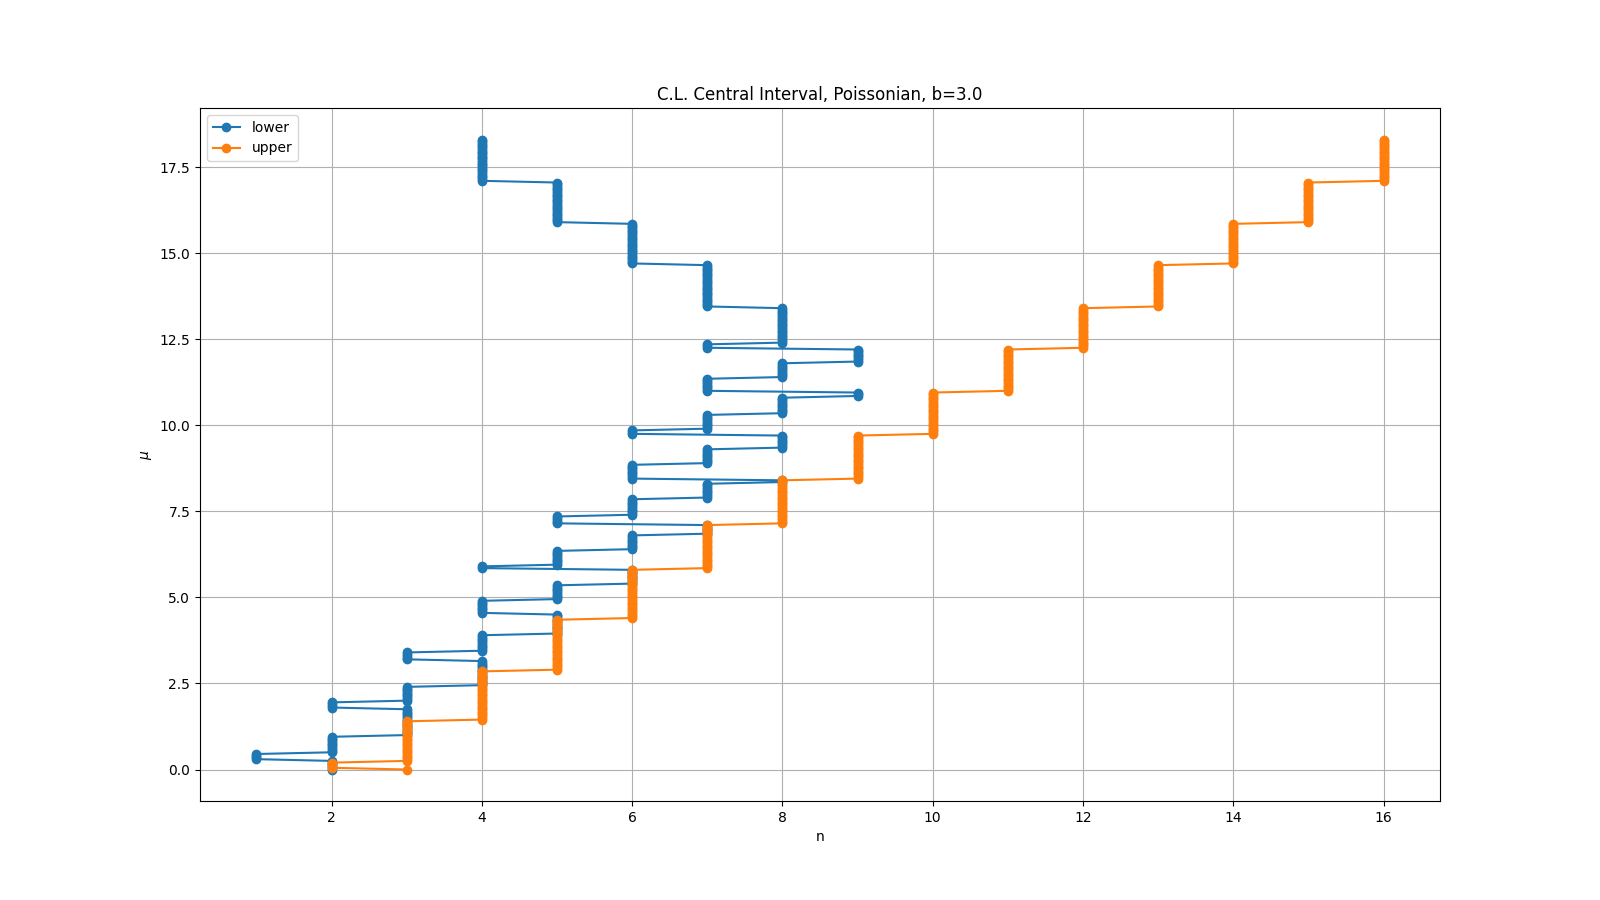
\includegraphics[width=.9\linewidth]{pr3_cl.png}
\end{center}

\section*{References}
\label{sec:org46451d5}
\bibliography{../../../References/Bibliography}
\bibliographystyle{unsrt}
\end{document}